\documentclass[hidelinks,12pt,dvipsnames,border=2pt]{standalone}
%\usepackage[top=0.7in, bottom=0.8in, left=1in, right=1in]{geometry}
\usepackage{tikz}
\usepackage{hyperref}
\usetikzlibrary{arrows}
\usetikzlibrary{shapes}
\usepackage{enumitem}
\usepackage{bm}
\usepackage{mathdots}
\usepackage{amsmath}
\usepackage{tcolorbox}
\usetikzlibrary{shadings}
\usetikzlibrary{decorations.pathreplacing}
\usepackage{helvet}
\usepackage{url}
\usepackage{graphicx}
\usetikzlibrary{arrows.meta,positioning,fit,calc}
\renewcommand{\familydefault}{\sfdefault}


\usetikzlibrary{arrows,decorations.pathmorphing,backgrounds,fit,positioning,shapes.symbols,chains}

\begin{document}
	
% trim=left botm right top
\begin{tikzpicture}

% manhattan
\node at (0,0) {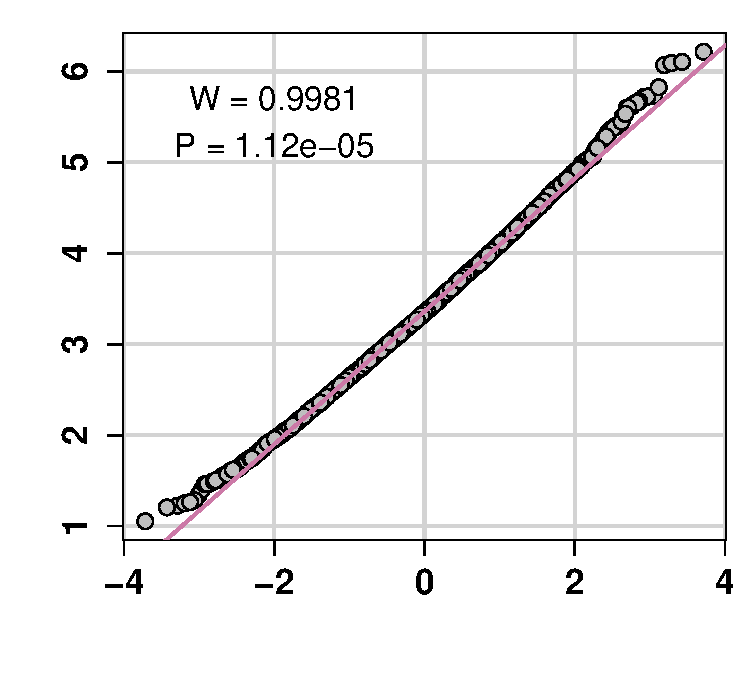
\includegraphics[width=\textwidth]{manhattan_QQ-plot_p10.pdf}};
\node at (0,-10.8) {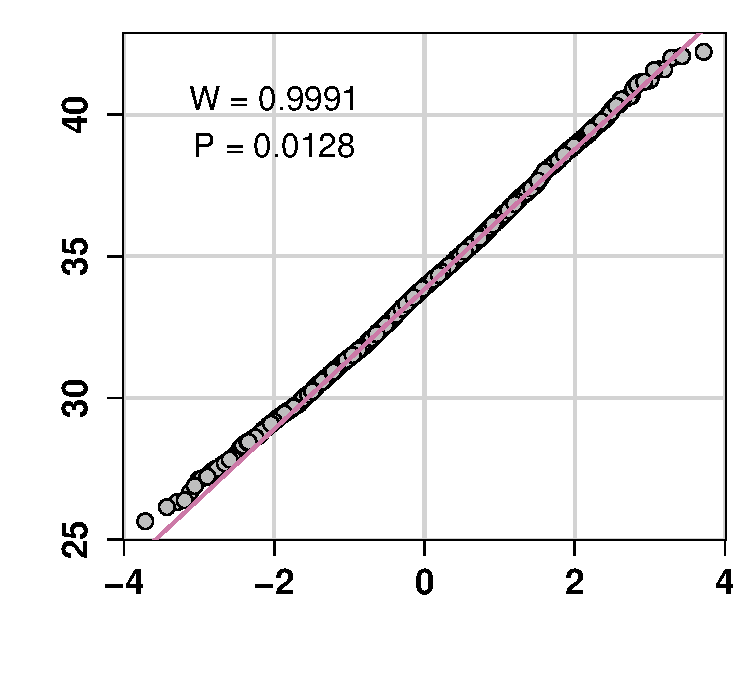
\includegraphics[width=\textwidth]{manhattan_QQ-plot_p100.pdf}};
\node at (0,-21.6) {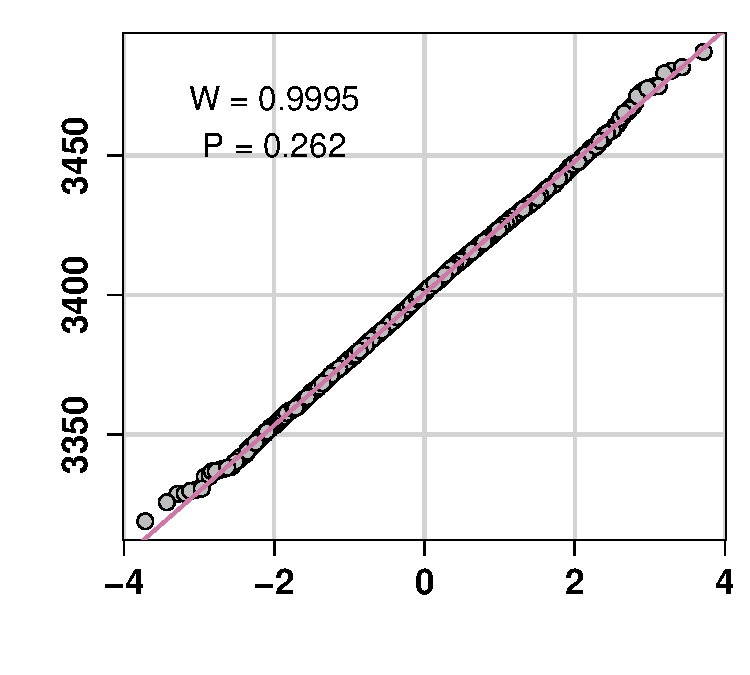
\includegraphics[width=\textwidth]{manhattan_QQ-plot_p10000.pdf}};

% euclidean
\node at (12.75,0) {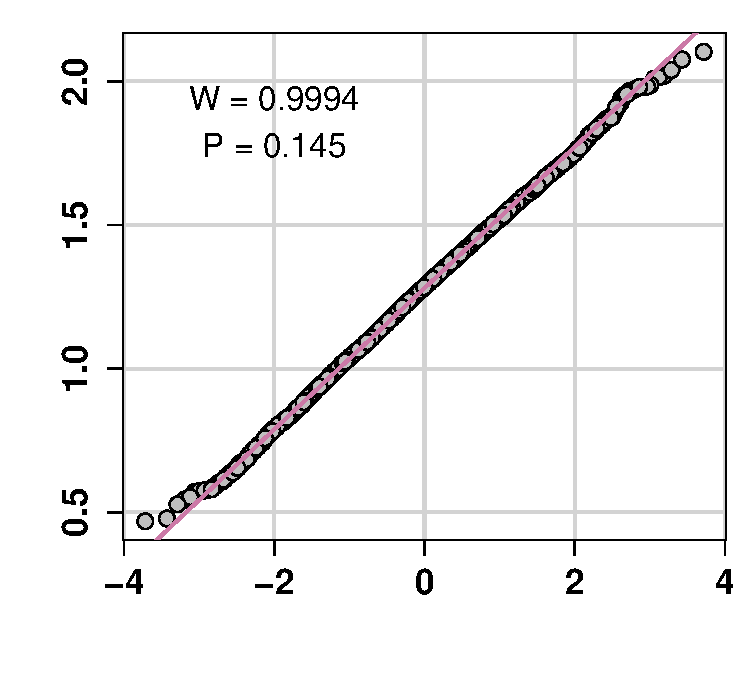
\includegraphics[width=\textwidth]{euclidean_QQ-plot_p10.pdf}};
\node at (12.75,-10.8) {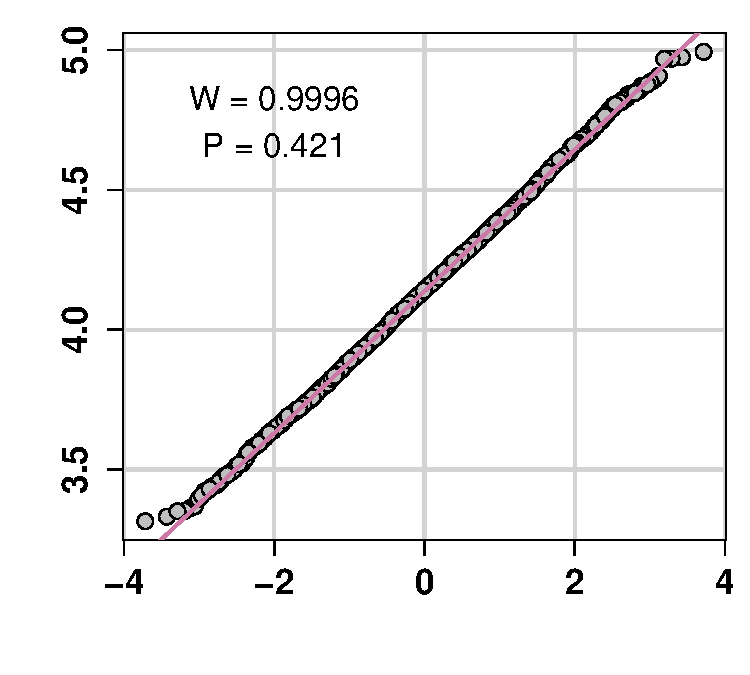
\includegraphics[width=\textwidth]{euclidean_QQ-plot_p100.pdf}};
\node at (12.75,-21.6) {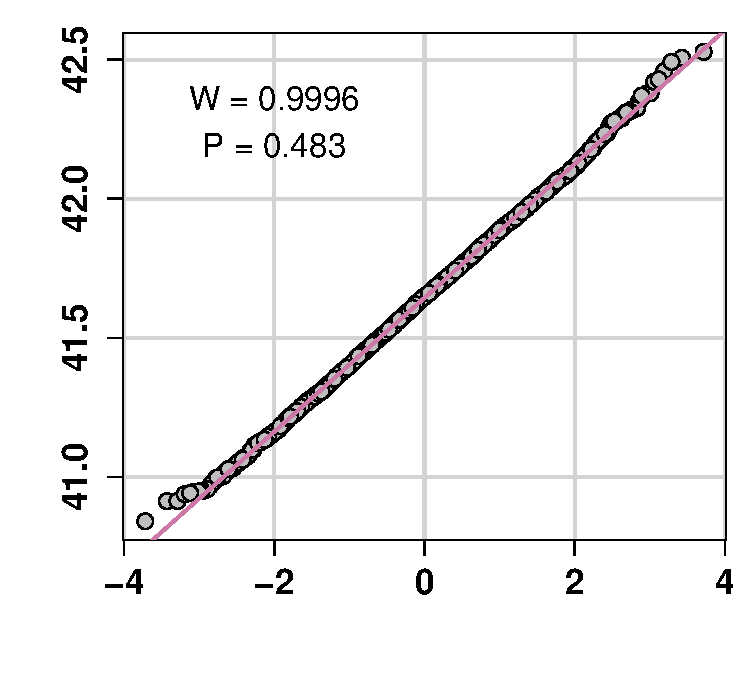
\includegraphics[width=\textwidth]{euclidean_QQ-plot_p10000.pdf}};

% labels

% p = 10
\node[draw,line width=0.25mm,fill=black!10,rotate=-90,text width=8.99cm,text height=1cm] at (19.81,0.93) {};
\node[xscale=1.9,yscale=1.9,rotate=-90] at (19.81,0.93) {10 attributes};

% p = 100
\node[draw,line width=0.25mm,fill=black!10,rotate=-90,text width=8.99cm,text height=1cm] at (19.81,-9.87) {};
\node[xscale=1.9,yscale=1.9,rotate=-90] at (19.81,-9.87) {100 attributes};

% p = 10000
\node[draw,line width=0.25mm,fill=black!10,rotate=-90,text width=8.99cm,text height=1cm] at (19.81,-20.67) {};
\node[xscale=1.9,yscale=1.9,rotate=-90] at (19.81,-20.67) {10000 attributes};

% axis titles

% vertical
\node[xscale=1.9,yscale=1.9,rotate=90] at (-6.6,-9.87) {Sample Quantiles};

% horizontal
\node[xscale=1.9,yscale=1.9] at (7.3,-27.5) {Theoretical Quantiles};

% manhattan
\node[xscale=1.9,yscale=1.9] at (0.9,6.4) {Manhattan};

% euclidean
\node[xscale=1.9,yscale=1.9] at (13.65,6.4) {Euclidean};
\end{tikzpicture}

\end{document}